
\documentclass[a4paper,11pt]{article}
\usepackage[a4paper, margin=8em]{geometry}

% usa i pacchetti per la scrittura in italiano
\usepackage[french,italian]{babel}
\usepackage[T1]{fontenc}
\usepackage[utf8]{inputenc}
\frenchspacing 

% usa i pacchetti per la formattazione matematica
\usepackage{amsmath, amssymb, amsthm, amsfonts}

% usa altri pacchetti
\usepackage{gensymb}
\usepackage{hyperref}
\usepackage{standalone}

% imposta il titolo
\title{Appunti Calcolo Numerico}
\author{Luca Seggiani}
\date{2025}

% disegni
\usepackage{pgfplots}
\pgfplotsset{width=10cm,compat=1.9}

% imposta lo stile
% usa helvetica
\usepackage[scaled]{helvet}
% usa palatino
\usepackage{palatino}
% usa un font monospazio guardabile
\usepackage{lmodern}

% tikz in sans
\tikzset{every picture/.style={/utils/exec={\sffamily}}}

\renewcommand{\rmdefault}{ppl}
\renewcommand{\sfdefault}{phv}
\renewcommand{\ttdefault}{lmtt}

% circuiti
\usepackage{circuitikz}
\usetikzlibrary{babel}

% disponi il titolo
\makeatletter
\renewcommand{\maketitle} {
	\begin{center} 
		\begin{minipage}[t]{.8\textwidth}
			\textsf{\huge\bfseries \@title} 
		\end{minipage}%
		\begin{minipage}[t]{.2\textwidth}
			\raggedleft \vspace{-1.65em}
			\textsf{\small \@author} \vfill
			\textsf{\small \@date}
		\end{minipage}
		\par
	\end{center}

	\thispagestyle{empty}
	\pagestyle{fancy}
}
\makeatother

% disponi teoremi
\usepackage{tcolorbox}
\newtcolorbox[auto counter, number within=section]{theorem}[2][]{%
	colback=blue!10, 
	colframe=blue!40!black, 
	sharp corners=northwest,
	fonttitle=\sffamily\bfseries, 
	title=Teorema~\thetcbcounter: #2, 
	#1
}

% disponi definizioni
\newtcolorbox[auto counter, number within=section]{definition}[2][]{%
	colback=red!10,
	colframe=red!40!black,
	sharp corners=northwest,
	fonttitle=\sffamily\bfseries,
	title=Definizione~\thetcbcounter: #2,
	#1
}

% disponi problemi
\newtcolorbox[auto counter, number within=section]{problem}[2][]{%
	colback=green!10,
	colframe=green!40!black,
	sharp corners=northwest,
	fonttitle=\sffamily\bfseries,
	title=Problema~\thetcbcounter: #2,
	#1
}

% disponi codice
\usepackage{listings}
\usepackage[table]{xcolor}

\definecolor{codegreen}{rgb}{0,0.6,0}
\definecolor{codegray}{rgb}{0.5,0.5,0.5}
\definecolor{codepurple}{rgb}{0.58,0,0.82}
\definecolor{backcolour}{rgb}{0.95,0.95,0.92}

\lstdefinestyle{codestyle}{
		backgroundcolor=\color{black!5}, 
		commentstyle=\color{codegreen},
		keywordstyle=\bfseries\color{magenta},
		numberstyle=\sffamily\tiny\color{black!60},
		stringstyle=\color{green!50!black},
		basicstyle=\ttfamily\footnotesize,
		breakatwhitespace=false,         
		breaklines=true,                 
		captionpos=b,                    
		keepspaces=true,                 
		numbers=left,                    
		numbersep=5pt,                  
		showspaces=false,                
		showstringspaces=false,
		showtabs=false,                  
		tabsize=2
}

\lstdefinestyle{shellstyle}{
		backgroundcolor=\color{black!5}, 
		basicstyle=\ttfamily\footnotesize\color{black}, 
		commentstyle=\color{black}, 
		keywordstyle=\color{black},
		numberstyle=\color{black!5},
		stringstyle=\color{black}, 
		showspaces=false,
		showstringspaces=false, 
		showtabs=false, 
		tabsize=2, 
		numbers=none, 
		breaklines=true
}

\lstdefinelanguage{javascript}{
	keywords={typeof, new, true, false, catch, function, return, null, catch, switch, var, if, in, while, do, else, case, break},
	keywordstyle=\color{blue}\bfseries,
	ndkeywords={class, export, boolean, throw, implements, import, this},
	ndkeywordstyle=\color{darkgray}\bfseries,
	identifierstyle=\color{black},
	sensitive=false,
	comment=[l]{//},
	morecomment=[s]{/*}{*/},
	commentstyle=\color{purple}\ttfamily,
	stringstyle=\color{red}\ttfamily,
	morestring=[b]',
	morestring=[b]"
}

% disponi sezioni
\usepackage{titlesec}

\titleformat{\section}
	{\sffamily\Large\bfseries} 
	{\thesection}{1em}{} 
\titleformat{\subsection}
	{\sffamily\large\bfseries}   
	{\thesubsection}{1em}{} 
\titleformat{\subsubsection}
	{\sffamily\normalsize\bfseries} 
	{\thesubsubsection}{1em}{}

% disponi alberi
\usepackage{forest}

\forestset{
	rectstyle/.style={
		for tree={rectangle,draw,font=\large\sffamily}
	},
	roundstyle/.style={
		for tree={circle,draw,font=\large}
	}
}

% disponi algoritmi
\usepackage{algorithm}
\usepackage{algorithmic}
\makeatletter
\renewcommand{\ALG@name}{Algoritmo}
\makeatother

% disponi numeri di pagina
\usepackage{fancyhdr}
\fancyhf{} 
\fancyfoot[L]{\sffamily{\thepage}}

\makeatletter
\fancyhead[L]{\raisebox{1ex}[0pt][0pt]{\sffamily{\@title \ \@date}}} 
\fancyhead[R]{\raisebox{1ex}[0pt][0pt]{\sffamily{\@author}}}
\makeatother

\begin{document}

% sezione (data)
\section{Lezione del 11-04-25}

% stili pagina
\thispagestyle{empty}
\pagestyle{fancy}

% testo
Riprendiamo il discorso dell'interpolazione polinomiale nella prospsettiva di arrivare all'interpolazione di Newton, a cui abbiamo accennato alla scorsa lezione.

Avevamo detto di avere $(x_0, y_0), (x_1, y_1), ..., (x_k, y_k)$, cioè $k + 1$ punti \textbf{distinti}, cioè con $x_i \neq x_j$, $\forall i \neq j$, tali per cui volevamo interpolarli con un polinomio di grado $k$.
Questo esisteva ed era unico appunto sotto l'ipotesi di punti distinti.


Avevamo qiundi visto le possibili base per la realizzazione di tale polinomio, di \textit{Vandermonde} e di \textit{Lagrange}.

\subsection{Differenze divise}
Avevamo poi introdotto la base di \textbf{Newton}, che definiva il polinomio del tipo:
$$
p_k (x) = \sum_{j = 0}^k a_j n_j(x) = \sum_{j = 0}^k f [ x_0, ..., x_j ] n_j(x)
$$
con:
\[
	\begin{cases}
			n_0(x) = 1 \\
			n_1(x) = x - x_0 \\
			n_2(x) = (x - x_0)(x - x_1) \\
			\vdots \\
			n_k(x) = (x - x_0) ... (x - x_{k + 1})
	\end{cases}
\]

Per la precisione, eravamo rimasti in attesa di definire i coefficienti $a_j$ del polinomio interpolante.

\par\smallskip

Cerchiamo di trovarli sfruttando la matrice di Vandermonde generalizzata (definizione 13.1):
$$
V = 
\begin{pmatrix}
	n_0(x_0) & n_1(x_0) & n_2(x_0) & ... & n_k(x_0) \\
	n_0(x_1) & n_1(x_1) & n_2(x_1) & ... & n_k(x_1) \\
	n_0(x_2) & n_1(x_2) & n_2(x_2) & ... & n_k(x_2) \\
	\vdots & & & & \vdots \\
	n_0(x_k) & n_1(x_k) & n_2(x_k) & ... & n_k(x_k) \\
\end{pmatrix}
$$
Applicando la definizione di base di Newton, si ottiene una forma del tipo:
$$
= \begin{pmatrix}
	1 & 0 & &  & ...0 \\ 
	1 & x_1 - x_0 & 0 & & ...0 \\ 
	1 & x_2 - x_0 & (x_2 - x_0)(x_2 - x_1) & 0 & ...0 \\ 
	\vdots & & & & \vdots \\
	1 & x_k - x_0 & (x_k - x_0)(x_k - x_1) & ... & (x_k - x_0) (x_k - x_1) ... (x_k - x_{k - 1}) \\ 
\end{pmatrix}
$$
cioè triangolare inferiore, e quindi risolvibile per sostituzione in avanti, imponendo:
$$
Va = y \, \Leftrightarrow \,
V \begin{pmatrix}
	a_0 \\ a_1 \\ a_2 \\ \vdots \\ a_k
\end{pmatrix}
=
\begin{pmatrix}
	y_0 \\ y_1 \\ y_2 \\ \vdots \\ y_k
\end{pmatrix}
$$

Svolgendo un paio di passaggi sella sostituzione in avanti, si ha:
\[
	\begin{cases}
		a_0 = y_0 \\
		y_0 + a_1 (x_1 - x_0) = y_1 \implies a_1 = \frac{y_1 - y_0}{x_1 - x_0} \\
		y_0 + (x_2 - x_0) \frac{y_1 - y_0}{x_1 - x_0} + (x_2 - x_0)(x_2 - x_1) a_2 = y_2 \implies a_2 = \frac{ \frac{y_2 - y_0}{x_2 - x_0} - \frac{y_1 - y_0}{x_1 - x_0} }{x_2 - x_1}
	\end{cases}
\]

Cioè si nota una forma comune per i coefficienti $a_j$

\par\smallskip

Questi coefficienti, che indichiamo con $a_j = f[x_0, ..., x_j]$ $\forall j$ si definiscono quindi per \textit{ricorsione}, e prendono il nome \textbf{differenze divise}.
Definiamo quindi la formula di ricorrenza:
\begin{definition}{Differenza divisa}
	Data una funzione $f: \mathbb{R} \rightarrow \mathbb{R}$, e dati $x_0, ..., x_{k - 1} \in \mathbb{R}$, con $x_i \neq x_j \, \forall i \neq j$, vogliamo una funzione $f[x]$ che rispetti:
	\[
		\begin{cases}
			f[x] = f(x), \quad k = 0 \\ \\
			f[x_0, x] = \frac{f(x) - f(x_0)}{x - x_0}, \quad k = 1 \\ \\
			f[x_0, x_1, x] = \frac{ \frac{f(x) - f(x_0)}{x - x_0} - \frac{f(x_1) - f(x_0)}{x_1 - x_0} }{x - x_1}, \quad k = 2 \\ \\
			f[x_0, ... , x_{k - 1}, x] = \frac{ f[x_0, ..., x] - f[x_0, ..., x_{k - 1}] }{ x - x_{k - 1} }, \quad \text{altrimenti}
		\end{cases}
	\]
	Chiamiamo questa funzione differenza divisa e la indichiamo come $f[x_0, ..., x ]$.
\end{definition}

Le differenze divise ricordano la forma del \textit{rapporto incrementale}, e anzi corrispondono esattamente a questo per $k = 1$, mentre per $k>1$ si può pensare ad un'approssimazione \textit{"grezza"}, o meglio \textit{finita},  delle derivate di ordine $k$, cioè:
\[
	\begin{cases}
		k = 0 : \quad f[x] = f(x)  \\
		k = 1 : \quad f[x_0, x] = \frac{f(x) - f(x_0)}{x - x_0} \approx \frac{df}{dx}(x_0) \\
		k = \ ? : \quad f[x_0, ... x_{k - 1}, x] = \frac{ f[x_0, ..., x] - f[x_0, ..., x_{k - 1}] }{ x - x_{k - 1} } \approx \frac{d^{k-2}f}{dx^{k-2}}(x_0) 
	\end{cases}
\]

\subsubsection{Proprietà delle differenze divise}
Possiamo trovare le seguenti proprietà delle differenze divise:
\begin{enumerate}
	\item $\forall P$ permutazione $\{i_0, ..., i_k\}$ di $\{0, ..., k \}$ vale:
		$$
			f[x_0, x_1, ..., x_k] = f[x_{i_0}, x_{i_1}, ..., x_{i_k}]
		$$
		cioè una permutazione dei $0, ..., k$ non cambia la differenza divisa;

	\item $f[x_0, ..., x_{k - 1}, x]$ è una funzione non definita in $x_0, ..., x_{k-1}$.
		Tuttavia, se $f \in C^1(I)$ con $I$ contenente $x_0, ..., x_k$, allora è prolungabile per continuità su tale intervallo;

	\item Se $f$ è non solo $C^1$, ma $f \in C^k(I)$, allora esiste $\epsilon$ tale che:
		$$
		\epsilon \in \left[ \min_{0 \leq i \leq k} x_i, \max_{0 \leq i \leq k} x_i \right]
		$$
		tale che:
		$$
		f[x_0, ..., x_k] = \frac{f^{(k)} (\epsilon) }{ k! } 
		$$ 
		Questa è una conseguenza del teorema di Lagrange.
\end{enumerate}

\subsubsection{Calcolo delle differenze divise}
Esiste un metodo piuttosto schematico per il calcolo delle differenze divise.
Dati $k + 1$ punti di interpolazione, si possono calcolare le differenze divise fino all'ordine $k$ secondo questo schema (posto $k = 3$), detto \textbf{quadro delle differenze divise}:

\begin{table}[H]
	\center 
	\begin{tabular} { c | c | p{2cm}  p{2cm} p{2cm} }
		$x$ & $f(x)$ & DD1 & DD2 & DD3 \\
		\hline
		$x_0$ & $f(x_0)$ & // & // & // \\
		$x_1$ & $f(x_1)$ & $f[x_0, x_1]$ & // & // \\
		$x_2$ & $f(x_2)$ & $f[x_0, x_2]$ & $f[x_0, x_1, x_2]$ & // \\
		$x_3$ & $f(x_3)$ & $f[x_0, x_3]$ & $f[x_0, x_2, x_3]$ & $f[x_0, x_1, x_2, x_3]$ \\
	\end{tabular}
\end{table}

Cioè a ogni passaggio completiamo una riga, da sinistra verso destra, con le differenze divise note a quel passaggio.
Notiamo che in verità le differenze divise che si trovano sulla diagonale sono le sole che compaiono effettivamente nel polinomio di Newton.

Supponendo di scrivere gli elementi della tabella come le entrate di una matrice $A = a{ij}$ triangolare inferiore, per calcolare una sua entrata $a_{ij}$ la formula da applicare è la seguente:
$$
a_{ij} = \frac{a_{i, j - 1} - a_{j - 1, j - 1}}{x_i - x}
$$

Poniamo infatti $A$:
$$
A = 
\begin{pmatrix}
	f(x_0) & & ... & & 0 \\
	f(x_1) & f[x_0, x_1] & & & & \\
	\vdots & f[x_0, x_2] & f[x_0, x_1, x_2] & & \vdots \\
	\vdots & \vdots & \vdots & & & \\
	f(x_k) &  f[x_0, x_k] & f[x_0, x_1, x_k] & ... & f[x_0, x_1, ..., x_k] \\
\end{pmatrix}
$$

\subsubsection{Esempio: quadro delle differenze divise}
Vediamo un caso pratico di quadro risolto:
\begin{table}[H]
	\center 
	\begin{tabular} { c | c | p{1cm}  p{1cm} p{1cm} }
		$x$ & $f(x)$ & DD1 & DD2 & DD3 \\
		\hline
		$0 $ & $ 3 $ & $ // $ & $ // $ & $ // $ \\
		$1 $ & $ 8 $ & $ 5 $ & $ // $ & $ // $ \\ 
		$2 $ & $ 15 $ & $ 6 $ & $ 1 $ & $ // $ \\
		$3 $ & $ 17 $ & $ 11 $ & $ 2 $ & $\frac{1}{2}$ \\
	\end{tabular}
\end{table}

A questo punto il polinomio sarà:
$$
p_3(x)
$$
$$
= f[x_0] + f[x_0, x_1] (x - x_0) + f[x_0, x_1, x_2] (x - x_0) (x - x_1) + f[x_0, x_1, x_2, x_3] (x - x_0) (x - x_1) (x - x_2) 
$$
$$
= 3 + 5 ( x - 0 ) + 1 ( x - 0 ) ( x - 1 ) + \frac{1}{2} ( x - 0 ) ( x - 1 ) ( x - 2 ) = \frac{1}{2}x^3 - \frac{1}{2}x^2 + 5x + 3
$$

Osserviamo che, nel caso in cui gli elementi di una colonna delle differenze divise siano tutti uguali, gli elementi delle colonne successive sono tutti nulli, e in particolare il grado del polinomio di interpolazione $p_k$ sarà $p_i$ con $i$ l'ultima colonna non nulla (cioè l'ordine dell'ultima differenza divisa non nulla). 

\subsubsection{Esempio: colonne nulle nel quadro}
Vediamo ad esempio il quadro delle differenze divise dove troviamo la situazione:
\begin{table}[H]
	\center 
	\begin{tabular} { c | c | p{1cm}  p{1cm} p{1cm} p{1cm} }
		$x$ & $f(x)$ & DD1 & DD2 & DD3 & DD4\\
		\hline
		$0 $ & $ 5 $ & $ // $ & $ // $ & $ // $ & $ // $ \\
		$-1 $ & $ 3 $ & $ 2 $ & $ // $ & $ // $ & $ // $ \\
		$2 $ & $ 3 $ & $ -1 $ & $ -1 $ & $ // $ & $ // $ \\
		$-2 $ & $ -9 $ & $ 7 $ & $-5 $ & $ 1 $ & $ // $ \\
		$3 $ & $ 11 $ & $ 2 $ & $ 0 $ & $ 1 $ & $ 0 $
	\end{tabular}
\end{table}

Come vediamo, alla colonna DD3 le differenze divise sono 1 e 1, ergo la differenza divisa in DD4 è nulla.
Questo significherà che il polinomio interpolante, sebbene sono stati presi $k + 1 = 5$ punti, da cui ci aspetteremo un polinomio di grado $k = 4$, ha invece grado $3$, cioè è:
$$
p_2(x) = 5 + 2 (x - 0) - 1 (x - 0)(x + 1) + 1 (x - 0)(x + 1)(x - 2) = x^3 - 2x^2 - x + 5
$$

\par\smallskip

Osserviamo infine che data una tabella di valori $(x_0, y_0), ..., (x_k, y_k)$ da interpolare, possiamo riordinarli come vogliamo nel quadro delle differenze divise.
Questo può essere utile a semplificare i calcoli.

\subsubsection{Esempio: riordinamento dei valori}
Poniamo di avere i seguenti dati:
\begin{table}[H]
	\center 
	\begin{tabular} { c | c }
		$x$ & $f(x)$ \\
		\hline
		0 & 2 \\
		1 & 1 \\
		$\alpha$ & 4 \\
		-1 & $3 \alpha + 1$ \\
		3 & 11 
	\end{tabular}
\end{table}
con $\alpha \in \mathbb{R} \setminus \{ 0, 1, -1, 3 \}$ e di chiederci quale deve essere il valore di $\alpha$ perché il polinomio interpolante abbia grado minimo.

Vediamo quindi di riordinare i dati in modo che i termini dipendenti da $\alpha$ vadano a finire in fondo alla tabella:
\begin{table}[H]
	\center 
	\begin{tabular} { c | c | p{1cm} p{1cm} p{1cm} p{1cm} }
		$x$ & $f(x)$ & DD1 & DD2 & DD3 & DD4\\
		\hline
		$0 $ & $ 2 $ & $ // $ & $ // $ & $ // $ & $ // $ \\
		$1 $ & $ 1 $ & $ -1 $ & $ // $ & $ // $ & $ // $ \\
		$3 $ & $ 11 $ & $ 3 $ & $ 2 $ & $ ...$ & $...$ \\
		$-1$ & $3 \alpha + 1$ & $1 - 3 \alpha$ & $\frac{3 \alpha - 2}{2}$ & $...$ & $...$ \\
		$\alpha$ & $4$ & $\frac{2}{\alpha}$ & $\frac{2 + \alpha}{\alpha(\alpha - 1)}$ & $...$ & $...$
	\end{tabular}
\end{table}

Alla colonna DD1 non abbiamo speranza di soddisfare la condizione di colonna tutta uguale (ci sono -1 e 3), mentre alla colonna DD2 possiamo provare ad imporre:
\[
	\begin{cases}
		\frac{3 \alpha - 2}{2} = 2 \implies \alpha = 2 \\
		\frac{2 + \alpha}{\alpha(\alpha - 1)} = 2 \implies \alpha = 2
	\end{cases}
\]
che quindi, per pura fortuna, corrisponde.
Possiamo allora prendere $\alpha = 2$ e completare il quadro:
\begin{table}[H]
	\center 
	\begin{tabular} { c | c | p{1cm} p{1cm} p{1cm} p{1cm} }
		$x$ & $f(x)$ & DD1 & DD2 & DD3 & DD4\\
		\hline
		$0 $ & $ 2 $ & $ // $ & $ // $ & $ // $ & $ // $ \\
		$1 $ & $ 1 $ & $ -1 $ & $ // $ & $ // $ & $ // $ \\
		$3 $ & $ 11 $ & $ 3 $ & $ 2 $ & $ // $ & $ // $ \\
		$-1$ & $3 \alpha + 1$ & $1 - 3 \alpha$ & $2$ & $0$ & $ // $ \\
		$\alpha$ & $4$ & $\frac{2}{\alpha}$ & $2$ & $0$ & $0$
	\end{tabular}
\end{table}
da cui il polinomio al solo grado 2:
$$
p_2(x) = 2 - x + 2x(x - 1) = 2x^2 - 3x + 2
$$

\subsubsection{Esempio: interpolazione di Newton}
A scopo di esempio, vediamo l'interpolazione di Newton della funzione:
$$
f\left(x\right)=\frac{x^{3}}{30}-\cos\left(\frac{3}{2}x\right)\ 
$$
Approssimata secondo la tabella di nodi:
\begin{table}[H]
	\center
	\begin{tabular} { c | p{1cm} p{1cm} p{1cm} p{1cm} p{1cm} p{1cm} p{1cm} }
		$x_j$ & $-5$ & $-4$ & $-1.9$ & $0$ & $2.3$ & $3.5$ & $5$ \\
		$y_j$ & $-4.51$ & $-3.09$ & $0.73$ & $-1$ & $1.36$ & $0.92$ & $3.82$
	\end{tabular}
\end{table}

Il polinomio si trova quindi prendendo le basi di Newton $n_j(x)$ e calcolando le differenze divise, come abbiamo visto finora:

\begin{table}[H]
	\center 
	\begin{tabular} { c | c | p{1cm} p{1cm} p{1cm} p{1cm} p{1cm} p{1cm} }
		$x$ & $f(x)$ & DD1 & DD2 & DD3 & DD4 & DD5 & DD6 \\
		\hline
		$-5 $ & $ -4.51 $ & $ // $ & $ // $ & $ // $ & $ // $ & $ // $ & $ // $ \\
		$-4 $ & $ -3.09 $ & $ 1.42 $ & $ // $ & $ // $ & $ // $ & $ // $ & $ // $ \\
		$-1.9 $ & $ 0.73 $ & $ 1.69 $ & $ 0.13 $ & $ // $ & $ // $ & $ // $ & $ // $ \\
		$0 $ & $ -1 $ & $ 0.7 $ & $ -0.18 $ & $ -0.16 $ & $ // $ & $ // $ & $ // $ \\
		$2.3 $ & $ 1.36 $ & $ 0.8 $ & $ -0.1 $ & $ -0.05 $ & $ 0.05 $ & $ // $ & $ // $ \\
		$3.5 $ & $ 0.92 $ & $ 0.64 $ & $ -0.1 $ & $ -0.04 $ & $ 0.03 $ & $ -0.01 $ \\
		$5 $ & $ 3.82 $ & $ 0.83 $ & $ -0.06 $ & $ -0.03 $ & $ 0.03 $ & $ \sim0 $ & $ \sim0$ 
	\end{tabular}
\end{table}

Da cui il polinomio:

$$
p_k(x) = -4.51 n_0(x) + 1.42 n_1(x) + 0.13 n_2(x) - 0.16 n_3(x) + 0.05 n_4(x) - 0.01 n_5(x)
$$

Vediamo quindi un grafico che mostra tale polinomio, sovraimposto alla funzione originale e ai nodi campionati:

\begin{center}
	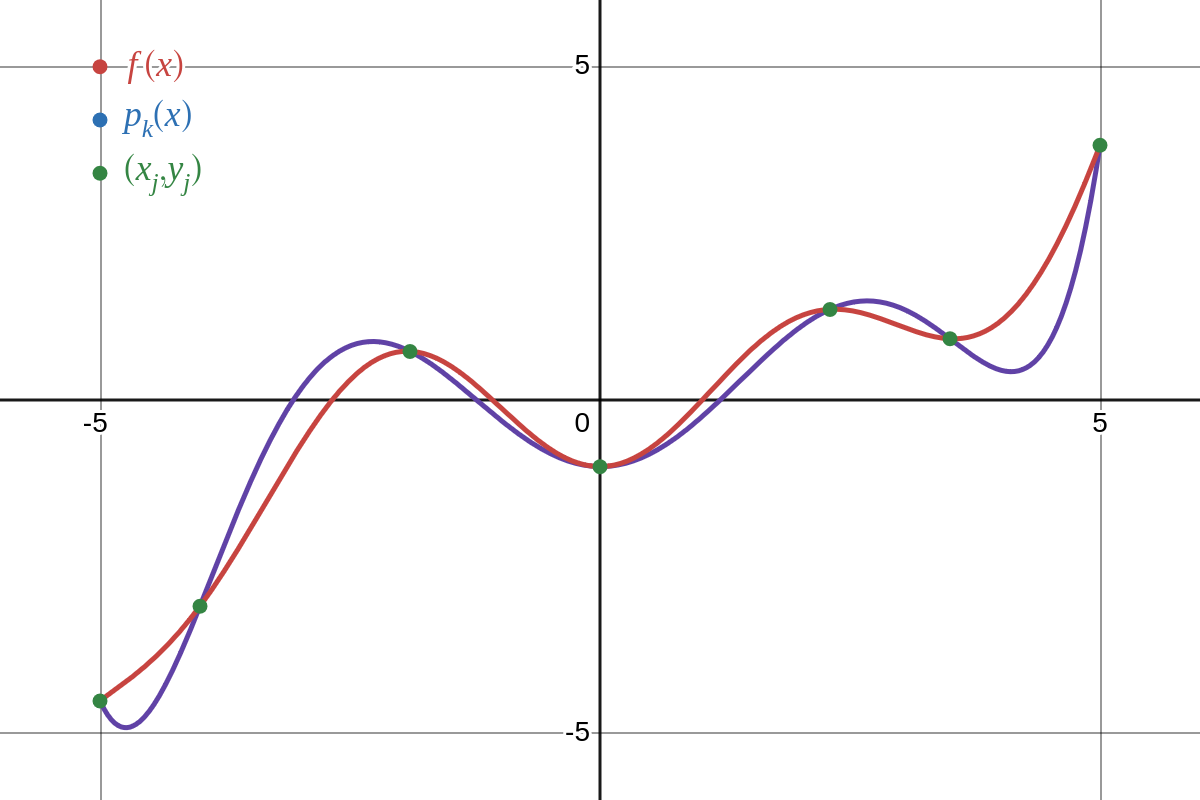
\includegraphics[scale=0.3]{../figures/newton_interpol.png}
\end{center}

Il grafico è stato realizzato con Desmos (\url{https://www.desmos.com/calculator/tavjyzgpd0}), assieme allo scorso esempio sull'interpolazione di Lagrange (\url{https://www.desmos.com/calculator/w2tx5n7jtp}, esempio 13.1.3).
Il calcolo al computer ci permette chiaramente di ottenere risultati più precisi, as esempio in questo caso a valutare il coefficiente della base di sesto grado (che svanisce approssimando alle prime 2 cifre decimali). 

\newpage

\subsection{Errore nell'approssimazione polinomiale}
Veniamo quindi alla valutazione dell'errore.
Vale il seguente teorema:
\begin{theorem}{Errore dell'approssimazione polinomiale}
	Presi $k + 1$ punti $x_0, ..., x_k$ con $x_i \neq x_j \, \forall i \neq j$.
	Sia $f: \mathbb{R} \rightarrow \mathbb{R}$ tale che $f \in C^{k + 1}(I)$ con $I \subseteq \mathbb{R}$ contenente $x_0, ..., x_k$.
	Se $p_k(x)$ è il polinomio di interpolazione di grado al più $k$ che interpola i punti $(x_0, f(x_0), ..., (x_k, f(x_k)))$ allora riguardo all'errore vale:
$$
f(x) - p_k(x) = \Pi(x) \frac{f^{(k + 1)}(\xi)}{(k + 1)!}
$$
con:
$$
\Pi(x) = \prod_{j = 0}^k (x - x_j)
$$
per un certo $\xi$ tale che:
$$
\xi \in \left[ \min_{0 \leq i \leq k} x_i \cup x, \max_{0 \leq i \leq k} x_i \cup x \right]
$$
\end{theorem}

Osserviamo quindi che conoscendo una stima di $|f^{k + 1}|$ e  di $|\Pi(x)|$ si può provare a stimare l'errore del polinomio di interpolazione quando si valuta $p_k(x)$ fuori dai nodi $\{ x_j \}_{j=0}^k$.

\subsection{Considerazioni ulteriori sull'approssimazione polinomiale}
Vediamo quindi alcune nozioni che riguardano sia l'approssimazione di Newton che quella di Lagrange, che abbiamo visto rispettivamente in 13.1.4 e 14.1, e 13.1.2 (e che riguardano in verità anche il metodo di approssimazione di Vandermonde visto in 13.1.1).

\subsubsection{Riassunto fra base di Newton e base di Lagrange}
Facciamo quindi un riassunto confrontando la base di Newton e la base di Lagrange.
\begin{table}[h!]
	\center 
	\begin{tabular} { c p{6cm} | p{6cm} }
		& \bfseries Newton & \bfseries Lagrange \\
		\hline
		\bfseries Base & $n_j(x) = (x - x_0) ... (x - x_{j - 1}) $ & $l_j(x) = \prod_{i \neq j}^k \frac{x - x_i}{x_j - x_i}$ \\
		\bfseries Coef. & $f[x_0, ... x_j]$ & $f(x_j) = y_j$ \\ & \\
		& Con la base di Newton, se si è calcolato $p_k(x)$ e si vuole $p_{k + 1}(x)$, basta calcolare $m_{k + 1}$ e $f[x_0, ..., x_{k}]$ da $f[x_0, ..., x_{k - 1}]$ &
		Con la base di Lagrange, per fare la stessa cosa bisogna ricalcolare tutti gli $e_j(x)$ \\ & \\
		& Il grado del polinomio si nota facilmente & Per trovare il grado del polinomio bisogna espandere nella base dei monomi
	\end{tabular}
\end{table}

Viene da sé che i metodi di Vandermonde, Lagrange e Newton restituiscono tutti lo stesso polinomio (se non in forma algebricamente diversa), in quanto il polinomio interpolante di grado minimo è l'unico che passa per i punti $(x_j, y_j)$ forniti.

\subsubsection{Fenomeno di Runge}
Vediamo un fenomeno che accumuna tutti i tipi di approssimazione polinomiale: presa una certa approssimazione di grado $k$ di una funzione $f(x)$, quindi un polinomio $p(x)$ passante per $k + 1$ punti campionati da $f(x)$, si potrebbe pensare che aumentando il valore di $k$ si otterrebbero approssimazioni via via più accurate.
Questo è giusto per quanto riguarda i punti interni, ma riguardo agli estremi dell'intervallo di approssimazione notiamo che la funzione di errore $r(x) = p(x) - f(x)$ ha un errore costante se non addirittura crescente al crescere di $k$.

Prendiamo ad esempio la funzione:
$$
f(x) = \frac{1}{1 + x^2} \quad \text{(versiera di Agnesi)}
$$
interpolata fra $-2$ e $2$ ad intervalli regolari, quindi preso $k$ interpolata sui nodi:
$$
x_k = -2 + \frac{4}{k}i, \quad i = 0, 1, ..., k
$$

Con $k = 4$, si ottiene il seguente polinomio interpolante:
\begin{center}
	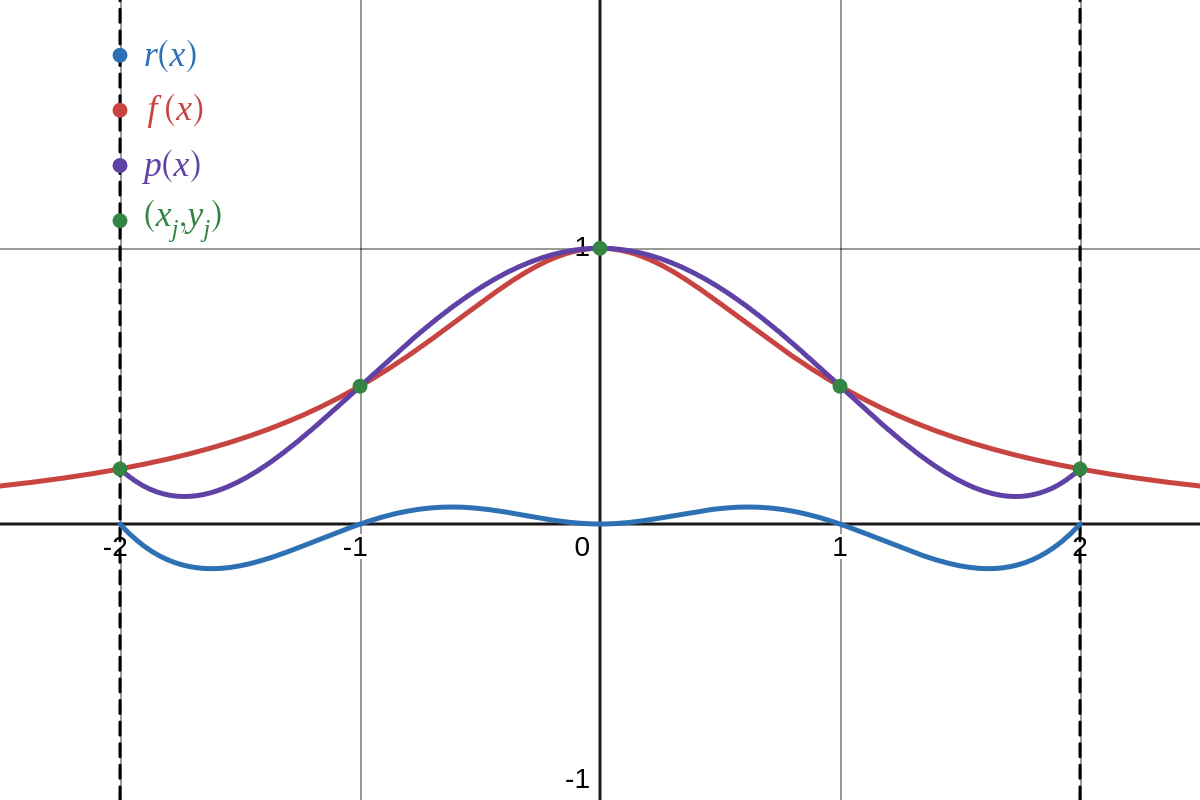
\includegraphics[scale=0.28]{../figures/runge_k4.png}
\end{center}

\newpage

Aumentando il grado a $k = 40$, quindi moltiplicando per 10, si ottiene invece il polinomio interpolante:
\begin{center}
	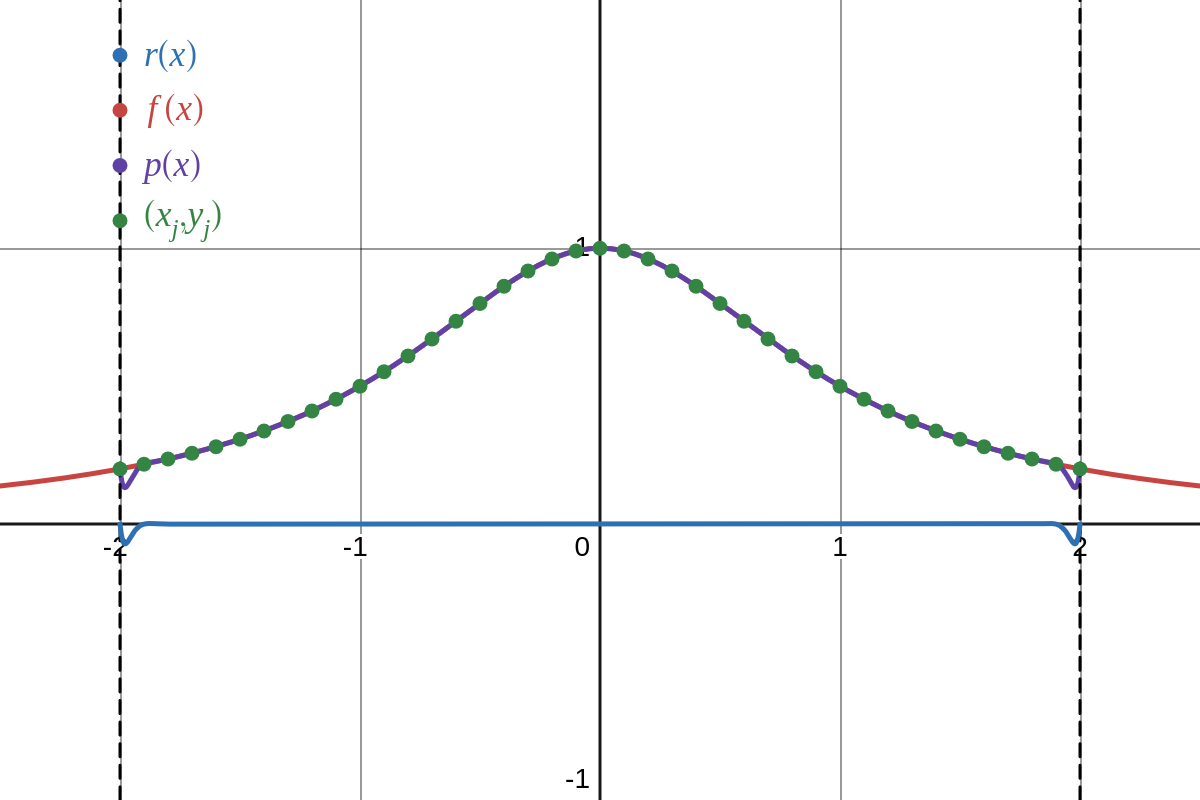
\includegraphics[scale=0.28]{../figures/runge_k40.png}
\end{center}
che è sì più accurato nei punti interni, ma ha comunque un certo errore in corrispondenza degli estremi $x = -2$ e $x = 2$.

Si può dimostrare che questo fenomeno permane al crescere di $k$, ergo aumentare il grado non corrisponde sempre a migliorare l'accuratezza dell'approssimazione.

\subsubsection{Nodi di Chebysev}
Un modo per migliorare l'accuratezza delle approssimazioni polinomiali, e sopratutto per evitare il fenomeno di Runge in prossimità degli estremi, può essere quello di cambiare i nodi presi, usando i cosiddetti \textbf{nodi di Chebyshev}.

\begin{definition}{Nodi di Chebyshev}
	Si chiamano nodi di Chebysev unitari gli $n$ punti $x_k$:
	$$
	x_k = \cos\left(\frac{\left(K+\frac{1}{2}\right)\pi}{n_{p}}\right), \quad k = 0, ..., n - 1
	$$
\end{definition}

\par\bigskip

\noindent
\begin{minipage}{\textwidth}
I nodi di Chebyshev corrispondono alle proiezioni sull'asse $x$ di punti equispaziati sulla parte superiore di una circonfenferenza unitaria, cioè sul grafico:
\begin{center}
	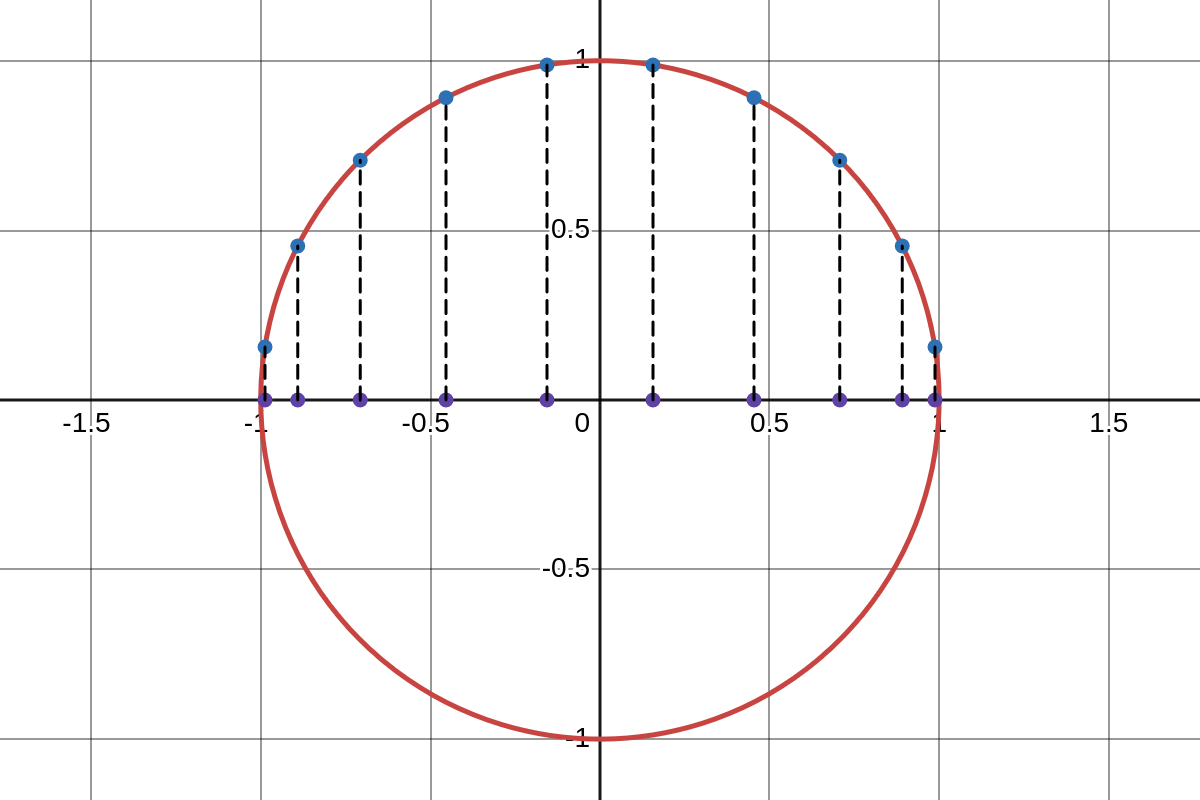
\includegraphics[scale=0.28]{../figures/chebyshev_nodes.png}
\end{center}
\end{minipage}

\par\bigskip

Utilizzando i nodi di Chebyshev nel calcolo del polinomio interpolante, si usano risultati molto più accurati.
Ad esempio, per l'approssimazione della stessa curva del paragrafo scorso, si ottiene che già con $k = 10$ il grafico ha la aspetto:
\begin{center}
	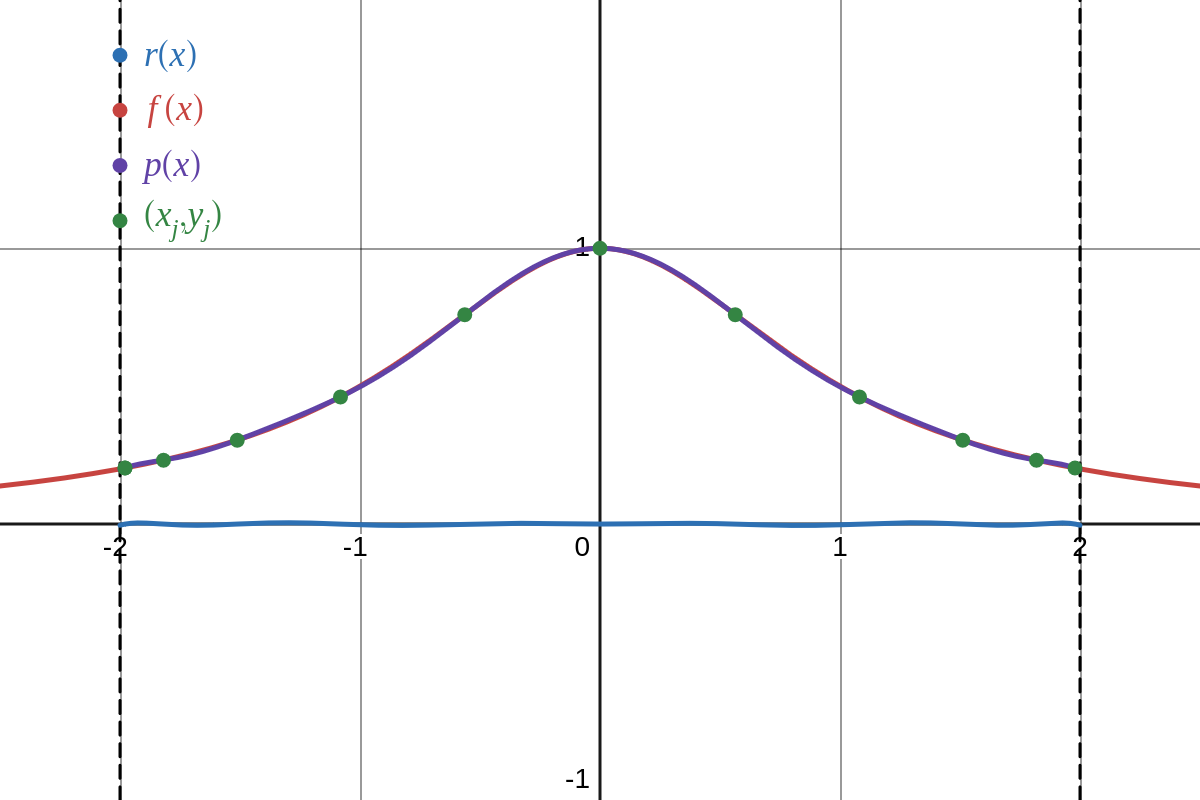
\includegraphics[scale=0.28]{../figures/runge_better.png}
\end{center}
da dove notiamo quindi che l'errore, sopratutto vicino agli estremi, è significativamente ridotto.

\subsection{Interpolazione osculatoria di Hermite}
Vediamo un altro metodo per interpolare polinomi.
Supponiamo di conoscere non soltanto ai nodi il valore della funzione, ma anche il valore della sua derivata.
In questo caso potremo costruire un polinomio in cui le valutazioni e quelle derivata equivalongono rispettivamente ai valori di $f$ e $f'$.
Questo potrebbe essere utile nel caso in cui conosciamo sia la posizione che la velocità di un corpo in certi istanti e vogliamo approssimarne la traiettoria.

Definiamo quindi:
\begin{definition}{Polinomio interpolante di Hermite }
	Dati $x_0, ..., x_k \in I \subseteq \mathbb{R}$ e $2k + 2$ valori $\{f(x_0), ..., f(x_k) \}$ e $\{ f'(x_0), ..., f'(x_k) \}$ di una certa funzione $f \in C^{1}(I)$, si dice polinomio interpolante di Hermite, per $f$ coi nodi $x_0, ..., x_k$, il polinomio $H_{2k + 1}(x)$ di grado al più $2k + 1$ tale che:
	$$
		H_{2k + 1}(x_j) = f(x_j), \quad H'_{2k + 1}(x_j) = f'(x_j), \quad \forall j = 0, ..., k
	$$
\end{definition}

Varrà quindi il seguente teorema:
\begin{theorem}{Esistenza del polinomio interpolante di Hermite}
	Se $x_i \neq x_j$ $\forall i \neq j$ allora esiste ed è unico il polinomio di Hermite $H_{2k + 1}$ per $f \in C^1(I)$. 
\end{theorem}
La dimostrazione di unicità si ha ipotizzando, per assurdo, che esista un secondo polinomio di hermite $S_{2k+1}$.
A questo punto si potrà definire la funzione di errore:
$$
R(x) = H_{2k + 1}(x) - S_{2k + 1}(x)
$$
Questà dovrà annullarsi fino al primo grado in $x_0, ..., x_k$, per cui dovrà essere divisiibile per:
$$
Q(x) = (x - x_0)^2 ... (x - x_k)^2
$$
Questo però significherebbe che $R(x)$, e quindi $H_{2k + 1}$ e $S_{2k + 1}$, dovrebbero essere almeno di grado $2k + 2$ (il grado di $Q(x)$), che viola le ipotesi. \qed 

\par\smallskip

Vediamo allora come trovare il polinomio $H_{2k + 1}$ vero e proprio.
Si potrebbe formulare un sistema lineare come è stato fatto nel caso della base canonica, che dava la matrice standard di Vandermonde.

In questo caso partiremo dall'ipotizzare riguardo a $H_{2k + 1}$:
$$
\mathrm{deg}(H_{2k + 1}) = 2k + 1, \quad H_{2k + 1} = a_0 + a_1 x + a_2 x^2 + ... + a_{2k + 1} x^{2k + 1} = \sum_{i = 0}^{2k + 1} a_i x^i
$$
e quindi imporre le condizioni:
\[
	\begin{cases}
		a_0 + a_1 x_0 + a_2 x_0^2 + ... + a_{2k + 1} x_0^{2k + 1} = f(x_0) \\	
		\vdots \\
		a_0 + a_1 x_k + a_2 x_k^2 + ... + a_{2k + 1} x_k^{2k + 1} = f(x_k) \\
		a_1 + 2 a_2 x_0 + ... + (2k + 1) a_{2k + 1} x_0^{2k} = f'(x_0) \\
		\vdots \\
		a_1 + 2 a_2 x_k + ... + (2k + 1) a_{2k + 1} x_k^{2k} = f'(x_k)
	\end{cases}
\]
da cui, volendo esprimere il sistema come $Va = y$, si ottiene la "matrice di Vandermonde":
$$
V = 
\begin{pmatrix}
	1 & x_0 & x_0^2 & ... & x_0^{2k + 1} \\	
	\vdots  & & & & \vdots \\
	1 & x_k & x_k^2 & ... & x_k^{2k + 1} \\
	0 & 1 & 2 x_0 & ... & (2k + 1) x_0^{2k} \\
	\vdots  & & & & \vdots \\
	0 & 1 & 2 x_k & ... & (2k + 1) x_k^{2k} 
\end{pmatrix}
$$

Spesso, però, questo procedimento non conviene in quanto si incontrano gli stessi problemi di malcondizionamento che avevamo incontrato anche nella matrice standard di Vandermonde.

\par\smallskip

Tipicamente allora si procede in maniera analoga all'interpolazione di Lagrange, ma generalizzata per ottenere le condizioni sulle derivate.
Più precisamente, cerchiamo un polinomio della forma:
$$
H_{2k + 1}(x) = \sum_{j = 0}^k h_{0j}(x) f(x_j) + \sum_{j = 0}^k h_{1j}(x) + f'(x_j)
$$

Avremo che $f(x_j)$ e $f'(x_j)$ sono chiaramente i dati del problema, che farano da coefficienti, mentre $h_{0j}(x)$ e $h_{1j}(x)$ saranno polinomi di grado $2k + 1$ tali che:
\begin{equation}
h_{0j}(x_i) =
\begin{cases}
	1, \quad i = j \\
	0, \quad i \neq j
\end{cases}, \quad
h'_{0j}(x_i) = 0  \quad \forall \, 0 \leq i \leq k
$$
$$
h_{1j}(x_i) = 0, \quad
h'_{1j}(x_i) =
\begin{cases}
	1, \quad i = j \\
	0, \quad i \neq j
\end{cases} \quad \forall \, 0 \leq i \leq k
\end{equation}
che possiamo interpretare come le condizioni imposte alle basi di Lagrange generalizzata al caso con la derivata prima.

Se valgono queste proprietà, infatti, si ha che:
$$
H_{2k + 1}(x_i) = \sum_{j = 0}^k h_{0j}(x_j) f(x_i) + \sum_{j = 0}^k h_{1j}(x_i) f'(x_j) = f(x_j) + 0 
$$
e rispetto alla derivata prima:
$$
H'_{2k + 1}(x_i) = \sum_{j = 0}^k h_{0j}'(x_i) f(x_j) + \sum_{j = 0}^k h'_{1j}f'(x_j) = 0 + f'(x_i)
$$
con in entrambi i casi, $\forall \, i = 0, ..., k$.

Osserviamo che come nel caso dell'interpolazione standard, stiamo rinunciando a cercare una rappresentazione di $H_{2k + 1}$ nella base dei monomi $\{ 1, x, ..., x^{2k + 1} \}$ e cerchiamo invece un'espressione rispetto alla base:
$$
	B_\text{Hermite} = \{ h_{01}(x), ..., h_{0k}(x), h_{10}(x), ..., h_{1k}(x) \}
$$
in cui i coefficienti delle combinazioni lineari sono:
$$
f(x_0), ..., f(x_k), f'(x_0), ..., f'(x_k)
$$

Il problema si riconduce quindi a trovare $h_{0j}(x)$, $h_{1j}(x)$ $\forall j$ che soddisfino le proprietà (3).

L'idea parte dall'\textit{ansatz} di cercare $h_{0j}$ e $h_{1j}$ della forma:
$$
h_{0j} = (Ax + B) e_j^2(x), \quad h_{1j} = (Cx + D) e_j^2(x)
$$
con $e_j(x)$ $j$-esimo polinomio in base di Lagrange, cioè:
$$
e_j(x) = \prod_{i \neq j}^k \frac{x - x_i}{x_j - x_i}
$$

Imponiamo quindi le proprietà (3) per ricavare $A, B, C, D$ di ogni $h_{0j}$ e $h_{1j}$.
\begin{itemize}
	\item $h_{0j}(x)$: avremo che la proprietà di grado zero è sempre rispettata finché:
		$$
		A x_j + B = 1
		$$
		in quanto $e_j^2(x_j)$ vale 1 o 0 esattamente come richiesto.
		Riguardo al primo grado, avremo invece:
		$$
		h_{0j}'(x_j) = A e_j^2 (x_j) + 2 (A x_j + B) e_j(x_j) e_j'(x_j) = 0
		$$
		dove si possono eliminare i termini $A x_j + B$ e $e_j(x_j)$, e quindi:
		$$
		A + 2 e_j'(x_j) = 0 \implies A = - 2 e_j'(x_j) 
		$$
		sostituendo in $Ax_j + B$ si trova allora:
		$$
		B = 1 + 2 e_j'(x_j) x_j
		$$
		da cui la funzione finale:
		$$
		h_{0j} = \left( 1 - 2 e_j'(x_j) (x - x_j) \right) e_j^2(x)
		$$

	\item $h_{1j}(x)$: avremo che la proprietà di grado zero è sempre rispettata finché:
		$$
		C x_j + D = 0
		$$
		in quanto $e_j^2(x_j)$ vale 1 soltanto in $x_j$, e lì vogliamo annullarlo.
		Riguardo al primo grado, avremo invece:
		$$
		h_{1j}' (x) = C e_j^2 (x) + 2 (Cx + D) e_j(x) e'_j(x) = 1
		$$
		dove si possono fare le stesse semplificazioni di sopra, e quindi:
		$$
		h_{1j}' = C e_j^2(x) \implies C = 1
		$$
		sostituendo in $Cx_j + D$ si trova allora:
		$$
		D = - x_j
		$$
		da cui la funzione finale:
		$$
		h_{1j}(x) = (x - x_j) e^2_j(x)
		$$
\end{itemize}

Abbiamo quindi ottenuto le due funzioni $h_{0j}$ e $h_{1j}$:
$$
	\begin{cases}
		h_{0j}(x) = \left( 1 - 2 e_j'(x_j) (x - x_j) \right) e_j^2(x) \\
		h_{1j}(x) = (x - x_j) e^2_j(x)
	\end{cases}
$$
ossia il polinomio interpolante di Hermite avrà la forma:
$$
H_{2k + 1}(x) = \sum_{j = 0}^k f(x_j) \left( 1 - 2 e_j'(x_j)(x - x_j) \right) e_j^2(x) + \sum_{j = 0}^k f'(x_j) (x - x_j) e_j^2(x)
$$

\subsubsection{Esempio: raccordo di binari}
Supponiamo di avere 2 binari e di volerli unire in maniera $C^1$, ovvero di voler trovare un polinomio $H_3(x)$ tale che:
\[
	\begin{cases}
		H_3(0) = 0 \\
		H_3(d) = L
	\end{cases}, \quad
	\begin{cases}
		H_3'(0) = 0 \\
		H_3'(d) = S
	\end{cases} 
\]

Il polinomio dovrà essere di grado 3 (le due condizioni alle derivate contano nel calcolo del grado).
Dobbiamo calcolare, prima di tutto, le basi di Lagrange:
$$
e_0(x) = \frac{x - d}{d}, \quad e_1(x) = \frac{x}{d}
$$
e sostituire quindi nelle formule per $h_{0j}(x)$ e $h_{1j}(x)$:
$$
h_{00}(x) = \left( 1 + 2\frac{x}{d} \right) \frac{(x - d)^2}{d^2}, \quad h_{01}(x) = \left( 1 - 2 \frac{x - d}{d} \right) \frac{x^2}{d^2}
$$
$$
h_{10}(x) = x \frac{(x - d)^2}{d^2}, \quad h_{11} = (x - d) \frac{x^2}{d^2}
$$
per cui otterremo:
$$
H_3(x) = 0 \cdot h_{00}(x) + L \cdot h_{01}(x) + 0 \cdot h_{10}(x) + S \cdot h_{11}(x) = L \left( 1 - 2 \frac{x - d}{d} \right) \frac{x^2}{d^2} + S (x - d) \frac{x^2}{d^2}
$$

Vediamo un esempio grafico:
\begin{center}
	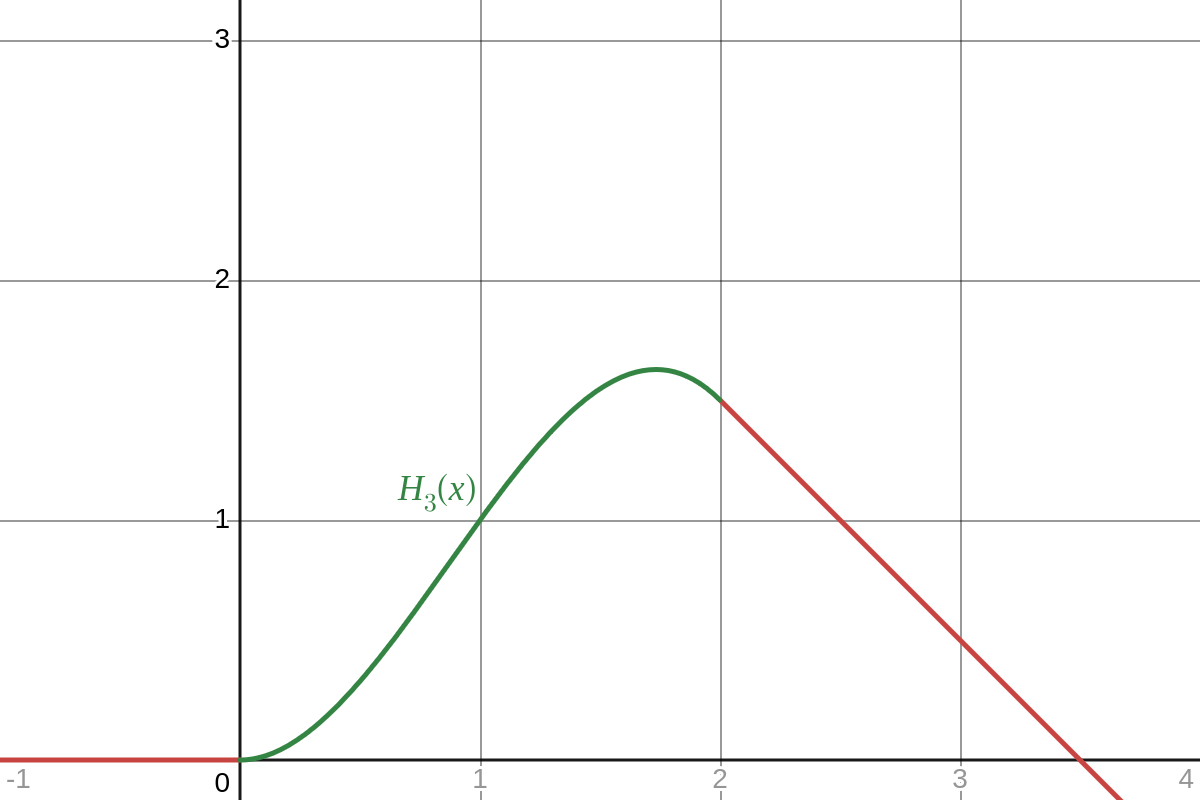
\includegraphics[scale=0.28]{../figures/tracks.png}
\end{center}

\subsubsection{Errore nell'approssimazione di Hermite}
Valutiamo quindi l'errore:
\begin{theorem}{Errore dell'approssimazione di Hermite}
	Data $f \in C^{2k + 2}(I)$ allora:
$$
f(x) - H_{2k + 1}(x) = \Pi^2 (x) \frac{f^{(2k + 1)(\xi)}}{(2k + 2)!}
$$
con le stesse definizioni del 14.1.
\end{theorem}

\end{document}
